\documentclass[12pt,titlepage]{article}
\usepackage[margin=1.25in]{geometry}
\usepackage{graphicx,amsmath,tabularx}

%% Variables definition
\newcommand{\vSubject}{Matematika 3}
\newcommand{\vSubtitle}{Minkowski, Hamming, and Chebyshev}
\newcommand{\vName}{Dicha Zelianivan Arkana}
\newcommand{\vNIM}{2241720002}
\newcommand{\vClass}{1i}
\newcommand{\vDepartment}{Information Technology}
\newcommand{\vStudyProgram}{D4 Informatics Engineering}

%% [START] Tikz related stuff
\usepackage{tikz}
\usetikzlibrary{svg.path,calc,shapes.geometric,shapes.misc}
\tikzstyle{terminator} = [rectangle, draw, text centered, rounded corners = 1em, minimum height=2em]
\tikzstyle{preparation} = [chamfered rectangle, chamfered rectangle sep=0.75em, draw, text centered, minimum height = 2em]
\tikzstyle{process} = [rectangle, draw, text centered, minimum height=2em]
\tikzstyle{decision} = [diamond, aspect=2, draw, text centered, minimum height=2em]
\tikzstyle{data}=[trapezium, draw, text centered, trapezium left angle=60, trapezium right angle=120, minimum height=2em]
\tikzstyle{connector} = [line width=0.25mm,->]
%% [END] Tikz related stuff

%% [START] Fancy header related stuff
\usepackage{fancyhdr}
\pagestyle{fancy}
\setlength{\headheight}{15pt} % compensate fancyhdr style
\fancyhead{}
\fancyfoot{}
\fancyfoot[L]{\thepage}
\fancyfoot[R]{\textit{\vSubject - \vSubtitle}}
\renewcommand{\footrulewidth}{0.4pt}% default is 0pt, overline for footer
%% [END] Fancy header related stuff

%% [START] Custom tabular command related stuff
\usepackage{tabularx}
\newcommand{\details}[2]{
    #1 & #2  \\
}
%% [END] Custom tabular command related stuff

%% [START] Figure related stuff
\newcommand{\image}[3][1]{
    \begin{figure}[h]
        \centering
        \includegraphics[#1]{#2}
        \caption{#3}
        \label{#3}
    \end{figure}
}
%% [END] Figure related stuff

\begin{document}
\begin{titlepage}
    \centering
    \vfill
    {\bfseries\LARGE
        \vSubject\\
        \vskip0.25cm
        \vSubtitle
    }
    \vfill
    
\includegraphics[width=6cm]{images/polinema-logo.png}
    \vfill
    {
        \textbf{Name}\\
        \vName\\
        \vskip0.5cm
        \textbf{NIM}\\
        \vNIM\\
        \vskip0.5cm
        \textbf{Class}\\
        \vClass\\
        \vskip0.5cm
        \textbf{Department}\\
        \vDepartment\\
        \vskip0.5cm
        \textbf{Study Program}\\
        \vStudyProgram
    }
\end{titlepage}

\section{Hamming Distance}

\subsection{Task 1}
\begin{figure}[h]
    \centering
    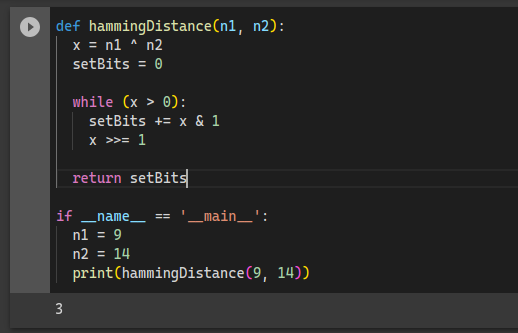
\includegraphics[width=.6\textwidth]{./images/hamming.png}
    \caption{The Hamming Distance implementation in Python}
\end{figure}

\subsection{Task 2}
\begin{figure}[h]
    \centering
    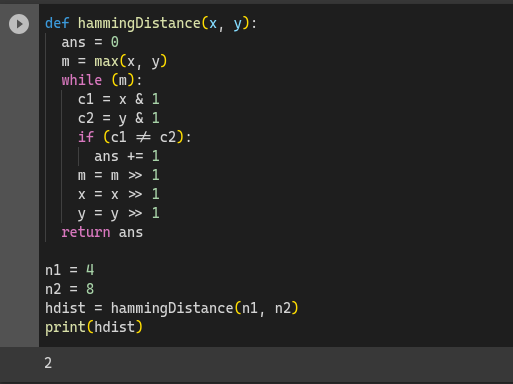
\includegraphics[width=.6\textwidth]{./images/hamming-2.png}
    \caption{The Hamming Distance alternative implementation in Python}
\end{figure}

\pagebreak

\subsection{Extra Task}
\begin{enumerate}
    \item {
        \begin{itemize}
            \item {
                BEEN and BEAN

                \begin{tabularx}{.5\textwidth}{|X|X|X|X|}
                    \hline
                    B & E & E & N \\
                    \hline
                    B & E & A & N \\
                    \hline
                    0 & 0 & 1 & 0 \\
                    \hline
                \end{tabularx}
                \begin{flalign*}
                    d &= 0 + 0 + 1 + 0 \\
                    d &= 1&&
                \end{flalign*}
            }
            \item {
                CEREAL and SERIAL

                \begin{tabularx}{.5\textwidth}{|X|X|X|X|X|X|}
                    \hline
                    C & E & R & E & A & L \\
                    \hline
                    S & E & R & I & A & L \\
                    \hline
                    1 & 0 & 0 & 1 & 0 & 0 \\
                    \hline
                \end{tabularx}
                \begin{flalign*}
                    d &= 1 + 0 + 0 + 1 + 0 + 0 \\
                    d &= 2&&
                \end{flalign*}
            }
            \item {
                10 and 15 in binary

                \begin{tabularx}{.5\textwidth}{|X|X|X|X|}
                    \hline
                    1 & 0 & 1 & 0 \\
                    1 & 1 & 1 & 1 \\
                    \hline
                    0 & 1 & 0 & 1 \\
                    \hline
                \end{tabularx}
                \begin{flalign*}
                    d &= 0 + 1 + 0 + 1 \\
                    d &= 2&&
                \end{flalign*}
            }
            \item {
                6 and 11 in binary

                \begin{tabularx}{.5\textwidth}{|X|X|X|X|}
                    \hline
                    0 & 1 & 1 & 0 \\
                    1 & 1 & 0 & 1 \\
                    \hline
                    1 & 0 & 1 & 1 \\
                    \hline
                \end{tabularx}
                \begin{flalign*}
                    d &= 1 + 0 + 1 + 1 \\
                    d &= 3&&
                \end{flalign*}
            }
        \end{itemize}
    }
\end{enumerate}

\pagebreak

\section{Minkowski}

\subsection{Task 3}

\begin{figure}[h]
    \centering
    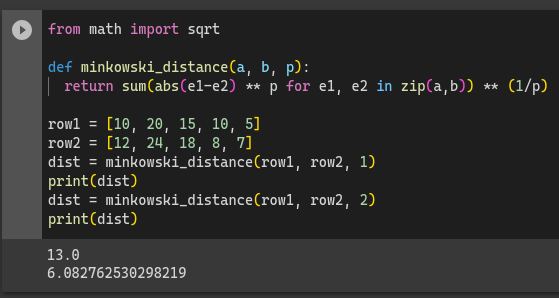
\includegraphics[width=0.6\textwidth]{./images/minkowski.png}
    \caption{Minkowski implementation in Python}
\end{figure}

\large{\textbf{Manual calculation}}
\begin{align*}
    row1 &= \begin{bmatrix}
        10 & 20 & 15 & 10 & 5
    \end{bmatrix} \\
    row2 &= \begin{bmatrix}
        12 & 24 & 18 & 8 & 7
    \end{bmatrix} \\
\end{align*}
\begin{itemize}
    \item {
        Euclidian
        \begin{align*}
            d &= \sqrt[2]{|10 - 12|^2 + |20 - 24|^2 + |15 - 18|^2 + |10 - 8)|^2 + |5 - 7|^2} \\
            d &= \sqrt[2]{4 + 16 + 9 + 4 + 4} \\
            d &= \sqrt[2]{37} \\
            d &= 6.082762530298219
        \end{align*}
    }
    \item {
        Manhattan / Cityblock
        \begin{align*}
            d &= \sqrt[1]{|10 - 12| + |20 - 24| + |15 - 18| + |10 - 8| + |5 - 7|} \\
            d &= \sqrt[1]{2 + 4 + 3 + 2 + 2} \\
            d &= \sqrt[1]{13} \\
            d &= 13
        \end{align*}
    }
\end{itemize}

\subsection{Task 4}
\subsection*{Minkowski}
Minkowski distance is a distance metric that is used to measure the distance between two points in a normed vector space. 
Minkowski can also be considered as a generalisation of Euclidean and Manhattan distance.

The Minkowski distance between two vectors $p$ and $q$ is defined as:
\begin{align*}
    d &= \sqrt[r]{\sum_{i=1}^{n} |x_i - y_i|^r}
\end{align*}
where $r$ is the order of the norm. When $r = 1$, this is equivalent to the Manhattan distance. 
When $r = 2$, this is equivalent to the Euclidean distance. 
When $r \rightarrow \infty$, this is equivalent to the Chebyshev distance.

An example of Minkowski Distance real world application is Brain Tumor Detection using Minkowski Distance and K-Nearest Neighbor (KNN) Algorithm.
The Minkowski distance is used to build a modified version of KNN algorithm to detect brain tumor.

\subsection*{Chebyshev}
Chebyshev distance is a distance metric that is used to measure the distance between two points in a normed vector space.
Chebyshev distance is also known as chessboard distance, maximum metric, or L-infinity metric. This is because the distance
between two points is the greatest of their differences along any coordinate dimension.

The Chebyshev distance between two vectors $p$ and $q$ is defined as:
\begin{align*}
    d_{\infty}(p, q) &= \lim_{r \rightarrow \infty} \sqrt[r]{\sum_{i=1}^{n} |x_i - y_i|^r} \\
    d_{\infty}(p, q) &= \max_{i=1}^{n} |x_i - y_i|
\end{align*}

An example of Chebyshev Distance real world application is Energy-Efficient Gossiping protocol (EEGossip).
This uses Chebyshev distance algorithm to determine the distance between two nodes in a network.
The goal of EEGossip is to minimize the energy consumption of the network.

\end{document}

